%%%%%%%%%%%%%%%%%%%%%%%%%%%%%%%%%%%%%%%%%%%%%%%%%%%%%%%%%%%%%%%%%%%%%%%%
% Preamble
%%%%%%%%%%%%%%%%%%%%%%%%%%%%%%%%%%%%%%%%%%%%%%%%%%%%%%%%%%%%%%%%%%%%%%%%
\documentclass[11pt]{article}
%
% Packages and other includes
% Pagination
\usepackage[letterpaper, margin=1.25in]{geometry}
%
% Graphics, floats, tables
\usepackage{graphicx, color, float, array}
%
% Hyperlinks
\usepackage{hyperref}
%
% AMS packages for equations, math symbols
\usepackage{amsmath, amssymb, braket}
%
% Bibliography
\usepackage[style=numeric,sorting=none]{biblatex}
\addbibresource{references.bib}
%
% Revision (see Makefile)
\newcommand{\Revision}{977be36}

%
% Definitions and settings
% Paragraph indent and spacing
\setlength{\parskip}{0.4\baselineskip}
\setlength{\parindent}{0in}
%
% Math mode version of "r" column type (requires array package)

%
% Title, authors, date
\title{\textbf{Simulating photoreaction pathways of TiO$_4$}}
\author{Brian Nguyen and Luke Nambi Mohanam}
\date{Chem 150L Winter 2018 \\ \today, Revision \Revision}
%
%
%%%%%%%%%%%%%%%%%%%%%%%%%%%%%%%%%%%%%%%%%%%%%%%%%%%%%%%%%%%%%%%%%%%%%%%%
% Main document
%%%%%%%%%%%%%%%%%%%%%%%%%%%%%%%%%%%%%%%%%%%%%%%%%%%%%%%%%%%%%%%%%%%%%%%%
%
\begin{document}

\maketitle

\begin{abstract}
  \noindent 
60 non-adiabatic molecular dynamics trajectories were run for
Ti(OH)$_4$ starting from vertical excitations into S$_1$ from
ground state molecular dynamics. The rare-event formation of
water from Ti(OH)$_4$ without any physisorbed water was
observed in the S$_1$ excited state, via a hydrogen transfer
. The immediate hop back to the ground state after the transfer 
indicates that the reaction is not well described by transition
state theory.
\end{abstract}

\section{Introduction}

Hydrogen fuel is considered as one of the future renewable sources
for transportation. However, the vast majority of industrial hydrogen
is produced from fossil fuels leading to significant carbon dioxide
emissions\cite{NI2007401}. One promising method is to use titanium dioxide
clusters that are able to catalytically split water in the presence of
light. The overall process is known to be ultrafast (within 1 ps),
making it suitable and important for molecular dynamics simulations
from first principles to be conducted; the time scale is small enough
to achieve reasonably accurate dynamics with modest computational
resources, and  ultrafast spectroscopic experiments benefit from
mechanistic insights from the simulations. 

Kazaryan and coworkers
suggest, based on transition state analysis, that photoexcited
Ti(OH)$_4$, representing the smallest possible hydroxylated 
titanium dioxide cluster, is able to extract a hydrogen from a
water molecule upon electronic excitation, producing 
a Ti(OH)$_3$(OH$_2$) radical and a OH radical.\cite{C5CP01812A}

\begin{figure}[H]
  \centering
  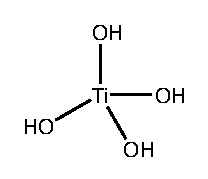
\includegraphics[scale=1.0]{tio4h4.eps}
  \caption{Tetrahedral structure of Ti(OH)$_4$}
  \label{fig:tio4h4}
\end{figure}

Muuronen and coworkers have in contrast performed non-adiabatic
molecular dynamics (NAMD) with a hydroxylated (TiO$_2$)$_4$
nanoparticle with physisorbed water.\cite{C6SC04378J} By
observing the dynamic time evolution of the electron-hole pair,
the simulation consistently matches with STM experiments. This
analysis using explicit dynamics is not captured in transition
state analysis. It was determined that localizing the excited
electron and the electron hole were important to catalysis.

We hypothesize that Ti(OH)$_4$, in the absence of other water
molecules, may spontaneously form free water molecules upon
electronic excitation. This would be 
one of the steps of a mechanism for water splitting by
Ti(OH)$_4$.
Rather than using the transition
state analysis employed by Kazaryan, we choose to employ
NAMD similar to Muuronen's work to capture the
non-adiabatic dynamics of this reaction.

\section{Methods}

\subsection{Statement of the Models}

Molecular potential energy surfaces (PES) are based on the Born-Oppenheimer (BO)
approximation which assumes the separation of the electronic and nuclear degrees
of freedom. However, this approximation breaks down whenever two or more
electronic states are strongly coupled\cite{C3CP51514A}, for
example by the nuclear velocity. One method to treat this
derivative coupling to nuclear postition
 is the non-adiabatic molecular dynamics (NAMD) within
the framework of the time-dependent Schr\"odinger equation. For each
nuclear configuration, \textbf{R}, the time-evolution of the electronic
wavefunction $|\psi(r|\textbf{R})\rangle$,

\begin{equation}
  i \frac{\partial}{\partial t}|\Psi(r|\textbf{R})\rangle
      = \hat{H}_{el}(t|\textbf{R})|\Psi(r|\textbf{R})\rangle.
\end{equation}

The time-dependent electronic Hamiltonian is defined as,

\begin{equation}
  \hat{H}_{\text{el}}(\textbf{r}|\textbf{R}(t)) = \
\hat{T}_{\text{e}}(\textbf{r}) +
\hat{V}_{\text{ee}}(\textbf{r}) + 
\hat{V}_{\text{ne}}(\textbf{r}|\textbf{R}(t))  + 
\hat{V}_{\text{nn}}(\textbf{r}|\textbf{R}(t))
\end{equation}

where $\hat{T}_{\text{e}}$ is the electronic kinetic energy, $\hat{V}_{\text{ee}}$ is the
electron-electron replusion, $\hat{V}_{\text{ne}}$ is the electron-nucleus attraction,
and $\hat{V}_{\text{nn}}$ is the nucleus-nucleus replusion. Meanwhile, the
evolution of the nucleus is simply the Newton's classical equations of
motion,

\begin{equation}
  \mathbf{F}_j(t) = m_j \mathbf{\"R}_j(t)
\end{equation}

where $\mathbf{F}_j$, $m_j$, and $\textbf{\"R}_j$ denotes the force, the mass, and
acceleration, respectively, of the $j$th nuclei
at time $t$. In the simulation of Ti(OH)$_4$, the forces are determined
with the fewest switches surface hopping (FSSH) method\cite{doi:10.1063/1.459170}
in the basis of the BO states. With the electronic wavefunction,

\begin{equation}
  |\Psi(t|\mathbf{R})\rangle = \sum_n c_n(t|\mathbf{R})|\Phi_n(\mathbf{R})\rangle,
\end{equation}

this can be inserted into the time-dependent Schr\"odinger equation and
yield the time-dependent amplitude vector \textbf{c},

\begin{eqnarray}
  i\dot{\mathbf{c}} & = & (\mathbf{H} - i\mathbf{W}) \\
  W_{mn} & = & \langle \Phi_m|\frac{\partial}{\partial t} \Phi_n \rangle
\end{eqnarray}

$W_{mn}$ is the nonadiabtic coupling of the two BO states $m$ and $n$.
A random number
 is generated to determine whether the molecule will hop between
one state to another. If the switch is accepted, the total
energy of the system
is conserved by scaling the momenta in the direction of the non-adiabatic coupling vector.
Otherwise for nuclear dynamics, the forces are computed where
$\mathbf{F}_j=-\frac{\partial E_m(\mathbf{R})}{\partial
\mathbf{R}_j}$
and then, the leapfrog Verlet algorithm is used to propagate the
nuclei,

\begin{eqnarray}
  \mathbf{P}(t_{i+1/2}) & = & \mathbf{P}(t_{i-1/2}) +  F(t_i)\Delta t \\
  \mathbf{Q}(t_{i+1}) & = & \mathbf{Q}(t_i) + \mathbf{M}^{-1}\mathbf{P}(t_{i+1/2}) 
\end{eqnarray}

where \textbf{P}, \textbf{Q}, and \textbf{M} are the nuclear momentum,
postion, and mass tensior, respectively.

\subsection{Computational Details}

The simulation of Ti(OH)$_4$ was computed on TURBOMOLE v7.2\cite{TURBOMOLE}
to sample the water splitting mechanism of Ti(OH)$_4$. The initial structures
are generated using ground state ab initio molecular dynamics (AIMD)
with PBE0\cite{doi:10.1063/1.478522} functional and def2-SVP basis set\cite{doi:10.1063/1.463096}.
At initial velocities of 2200K and 3200K, 30 trajectories were computed
at each temperature using 1 fs timestep (40 a.u.). Each trajectory ran
for a total of 250 fs. At every 85 fs, the coordinates of
the Ti(OH)$_4$ were extracted to run NAMD simulations with time-dependent
density functional theory and FSSH starting in the $S_1$ state,
simulating a vertical excitation. The same
PBE0\cite{doi:10.1063/1.478522} functional and def2-SVP basis\cite{doi:10.1063/1.463096}
were used. The NAMD simulations ran until the systems hopped to the $S_0$
ground state and the nonradiative excited state lifetime was determined by
the log-linear regression of the excited state population defined as,

\begin{equation}
  \rho^{\text{av}}_{11}(t) = \frac{1}{N_{\text{ensemble}}}\sum_{k\in ensemble}n_k(t)
\end{equation}

where $n_k=0$ means the simulation is at the ground state and $n_k=1$ is at
the excited state. The trajectories were visualized with the
MOLDEN package.

\section{Results}

A total of 60 NAMD simulations were performed and out of the 60,
only 7
trajectories revealed the formation of water. Of these trajectories,
only one showed a complete dissociation of water from the Ti(OH)$_4$
cluster as seen in Fig \ref{fig:snaps}. The overall reaction is
shown in Fig \ref{fig:reaction}. There is a hydrogen transfer in
this reaction, which with the electronic rearrangement produces
a Ti=O double bond and a water molecule.

\begin{figure}[H]
  \centering
  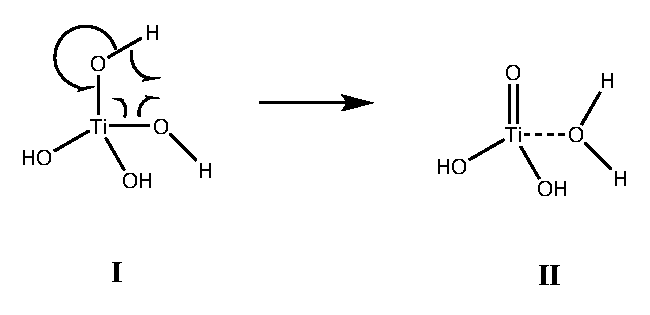
\includegraphics[scale=0.6]{reaction.eps}
  \caption{Reaction mechanism observed for Ti(OH)$_4$(I) to form
water(II).}
  \label{fig:reaction}
\end{figure}

For the trajectory that produced a free water molecule, the water 
formation and split from
Ti(OH)$_4$ took a total of 516 fs. The water appeared when the OH stretch
became vibrationally active and the hydrogen atom transfer from the OH ligand
to another OH ligand from Fig \ref{fig:snaps}. This suggested that the
vibrational nuclear degrees of freedom to be mainly responsible for
the excited states deactivation.


\begin{figure}[H]
  \centering
  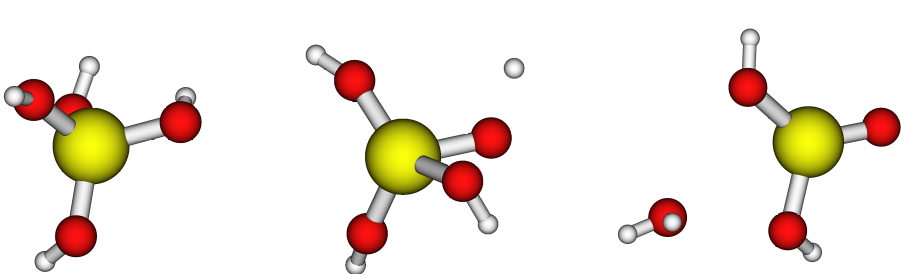
\includegraphics[scale=0.35]{tio2_snaps.png}
  \caption{Snapshots of the Ti(OH)$_4$ simulation taken at 0 fs (left),
    392 fs (middle), and 516 fs (right).}
  \label{fig:snaps}
\end{figure}

The rest of the trajectories did not undergo any reaction in the
excited state before hopping back to the ground state. The decay 
is plotted in fig \ref{fig:pop}.

\begin{figure}[H]
  \centering
  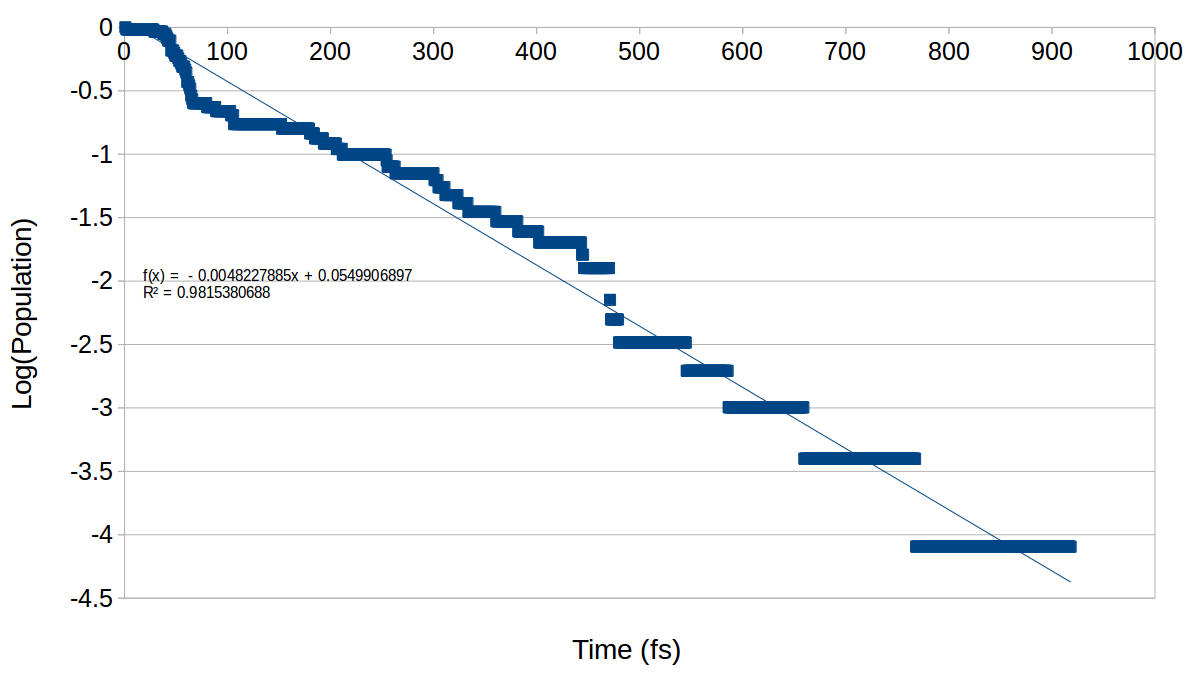
\includegraphics[scale=0.23]{pop_analysis.png}
  \caption{NAMD simulation of Ti(OH)$_4$ starting at the $S_1$ state
    Franck-Condon geometry that show the nonradiative excited state lifetime
  by the natural log-linear regression of the excited state population.}
  \label{fig:pop}
\end{figure}

In Fig \ref{fig:pop}, the population analysis of the 60 NAMD simulations
starting from the $S_1$ state Franck-Condon geometry with random nuclear
velocities showed that the nonradiative excited state lifetime is
approximately 207 fs.

\begin{figure}[H]
  \centering
  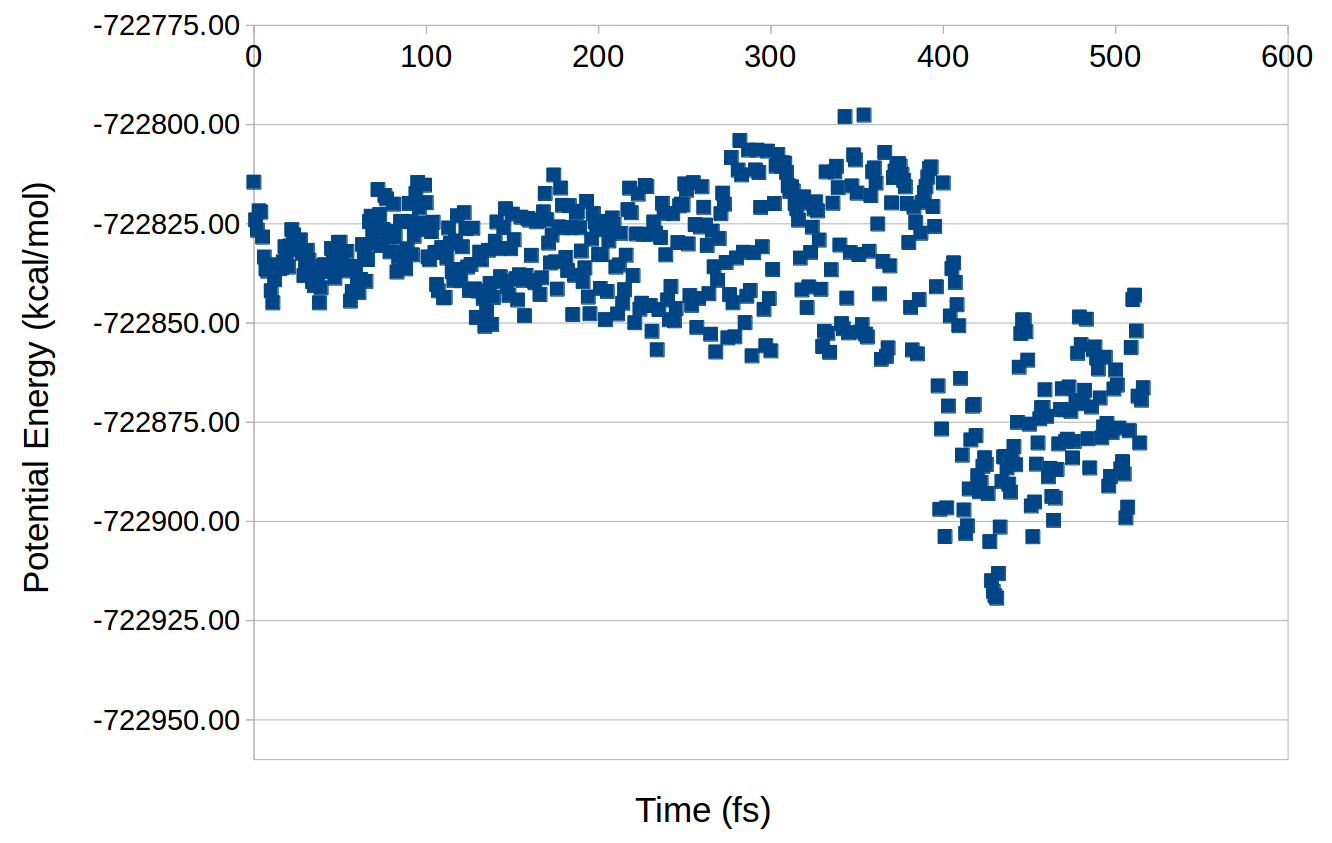
\includegraphics[scale=0.23]{egy.png}
  \caption{The potential energy of the Ti(OH)$_4$ system transitioning
    between the $S_1$ excited state and the $S_0$ ground state.}
  \label{fig:energy}
\end{figure}

In Fig \ref{fig:energy}, the transition from the $S_1$ state to the $S_0$
state is approximately a difference of 25 kcal/mol. This transition appears
to happen at approximately 400 fs. Prior to the transition is the
vibrationally active OH stretch beginning at approximately 300 fs. This
relative energy difference captured from the NAMD simulation appears to match
fairly close to the CCSD(T) relative potential energies of the reaction
of H$_2$O with Ti(OH)$_4$ at the excited state\cite{C5CP01812A} which is
approximately 34 kcal/mol.

Due to the small number of trajectories, the population analysis
for the products of photo-excitation of Ti(OH)$_4$ is skewed. 1
in 10 trajectories is observed to form water, but only 1 
in 60 trajectories forms a free water molecule.

\section{Conclusions}

In summary, our NAMD simulation of Ti(OH)$_4$ demonstrate a
rare-event
mechanism for the formation of a free water molecule upon
photo-excitation to the S$_1$ state. The formation of water
molecules is more frequent, and may
the more important reaction pathway. Analysis suggests that the 
nonradiative
transition from the $S_1$ to $S_0$ state mainly depends on the nuclear
velocity in their vibrational motion. 
In addition, the transfer of hydrogen
appears to only happen in the excited states and not in the ground state.
This transfer leads to the formation of water and to an
immediate non-radiative transition
from the $S_1$ excited state to the $S_0$ ground state. 

\printbibliography

\end{document}
